\documentclass[a4paper,
fontsize=11pt,
%headings=small,
oneside,
numbers=noperiodatend,
parskip=half-,
bibliography=totoc,
final
]{scrartcl}

\usepackage{synttree}
\usepackage{graphicx}
\setkeys{Gin}{width=.8\textwidth} %default pics size

\graphicspath{{./plots/}}
\usepackage[ngerman]{babel}
\usepackage[T1]{fontenc}
%\usepackage{amsmath}
\usepackage[utf8x]{inputenc}
\usepackage [hyphens]{url}
\usepackage{booktabs} 
\usepackage[left=2.4cm,right=2.4cm,top=2.3cm,bottom=2cm,includeheadfoot]{geometry}
\usepackage{eurosym}
\usepackage{multirow}
\usepackage[ngerman]{varioref}
\setcapindent{1em}
\renewcommand{\labelitemi}{--}
\usepackage{paralist}
\usepackage{pdfpages}
\usepackage{lscape}
\usepackage{float}
\usepackage{acronym}
\usepackage{eurosym}
\usepackage[babel]{csquotes}
\usepackage{longtable,lscape}
\usepackage{mathpazo}
\usepackage[normalem]{ulem} %emphasize weiterhin kursiv
\usepackage[flushmargin,ragged]{footmisc} % left align footnote

\usepackage{listings}

\urlstyle{same}  % don't use monospace font for urls

\usepackage[fleqn]{amsmath}

%adjust fontsize for part

\usepackage{sectsty}
\partfont{\large}

%Das BibTeX-Zeichen mit \BibTeX setzen:
\def\symbol#1{\char #1\relax}
\def\bsl{{\tt\symbol{'134}}}
\def\BibTeX{{\rm B\kern-.05em{\sc i\kern-.025em b}\kern-.08em
    T\kern-.1667em\lower.7ex\hbox{E}\kern-.125emX}}

\usepackage{fancyhdr}
\fancyhf{}
\pagestyle{fancyplain}
\fancyhead[R]{\thepage}

%meta
%meta

\fancyhead[L]{I. Frank \\ %author
LIBREAS. Library Ideas, 30 (2016). % journal, issue, volume.
\href{http://nbn-resolving.de/
}{}} % urn
\fancyhead[R]{\thepage} %page number
\fancyfoot[L] {\textit{Creative Commons BY 3.0}} %licence
\fancyfoot[R] {\textit{ISSN: 1860-7950}}

\title{\LARGE{Fortschritt durch Rückschritt -- vom Bibliothekskatalog zum Denkwerkzeug \\ Eine Idee}} %title %title
\author{Ingo Frank} %author

\setcounter{page}{1}

\usepackage[colorlinks, linkcolor=black,citecolor=black, urlcolor=blue,
breaklinks= true]{hyperref}

\date{}
\begin{document}

\maketitle
\thispagestyle{fancyplain} 

%abstracts
\begin{abstract}
Der Text zeigt anhand einer essayistisch selektiven Rückschau in die
Zeit vor den Digital Humanities bibliotheks- und
informationswissenschaftliche Ansätze zur Entwicklung hypertextueller
Werkzeuge für Bibliographie-Verwaltung und Strukturierung des
wissenschaftlichen Diskurses - eine zukunftsweisende Idee für eine
digitale Geisteswissenschaft zur Unterstützung geisteswissenschaftlicher
Denkarbeit jenseits von reinem `distant thinking'.
\end{abstract}

%body
\enquote{What would I recommend to a young visionary today? Very
straightforward, learn to live with short term goals and not delegate.
{[}. . . {]} {[}I{]}f I had been able to hold it together and not try to
overstretch and overgrab and managed short term goals better, things
would have been very different.}

--- Ted Nelson (Nelson, 1996)

\section*{Einleitung}\label{einleitung}

Die Aufbereitung der Zusammenhänge der Forschungsliteratur in
elektronischen Bibliothekskatalogen wird bis heute nicht den
Anforderungen von (Geistes)Wissenschaftlern gerecht (Zumstein und Stöhr,
2015; Chambers, 2013). Der Bedarf für Annotations- und
Hypertextwerkzeuge zur Strukturierung des wissenschaftlichen Diskurses
in der Fachliteratur wurde bereits vor dem Aufkommen der Digital
Humanities in der Informationswissenschaft erkannt (Buckingham Shum u.
a., 2007) und entsprechende Ansätze zur Modellierung des
wissenschaftlichen Diskurses in der Forschungsliteratur wurden
entwickelt (Mancini und Shum, 2006; Neil, 2010). Im Prinzip gehen diese
Entwicklungen zurück auf Ted Nelsons Vision eines
Hypertext-Arbeitsplatzes (Nelson, 1965) zur Erfassung und Verwaltung
aller für ein Forschungsprojekt relevanter Dokumente (Nelson u. a.,
2007).

\section*{Vom
Bibliothekskatalog\ldots{}}\label{vom-bibliothekskatalog}

Nelson (1965) stellt sein Hypertext-System exemplarisch als digitalen
Arbeitsplatz eines Historikers vor (siehe Abb. 1). Zur Vernetzung der
Forschungsliteratur werden Hypertext-Links verwendet. Zur Einbindung von
Zitationen und Material aus Archivquellen wird Transklusion eingesetzt.
Durch typisierte Links können Provenienz von Primär- und Sekundärquellen
annotiert werden.

\begin{figure}
\centering
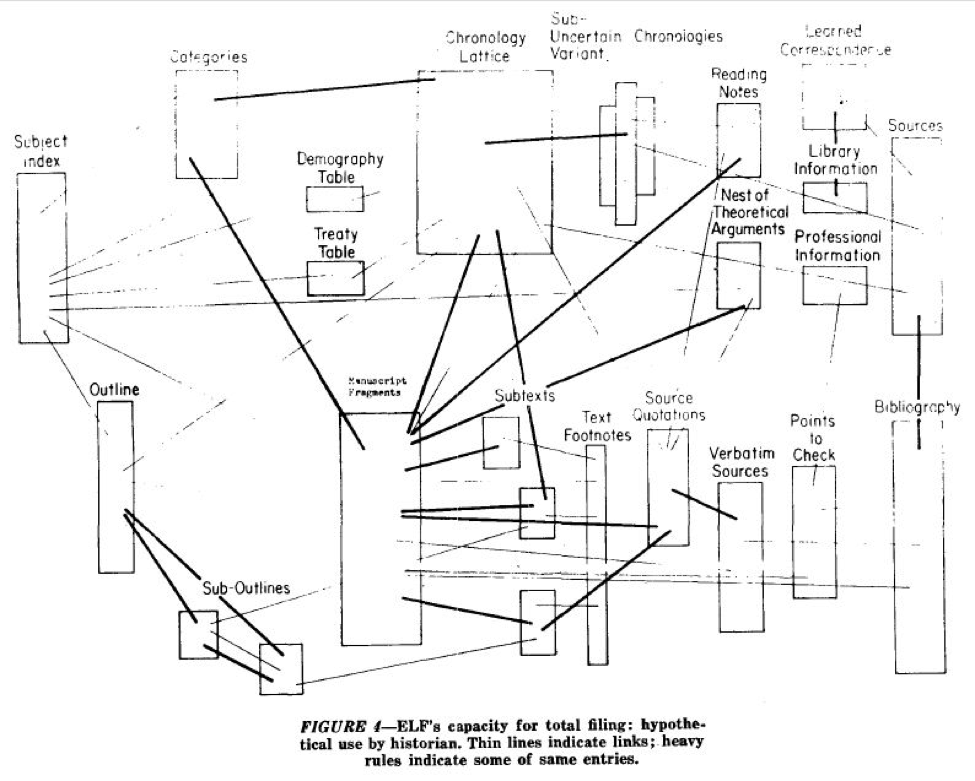
\includegraphics{img/abb1.png}
\caption{Diagramm der Verlinkung und Transklusion der
Forschungsliteratur für den Hypertext-Arbeitsplatzes eines Historikers
(ursprünglich in Nelson, 1965) (aus Nelson u. a., 2007)}
\end{figure}

Die Idee ist nun, durch schrittweise Umsetzung (Hodel, 2013) teilweise
alter bibliotheks- und informationswissenschaftlicher Ansätze einen
modernen Bibliothekskatalog als Arbeitswerkzeug für die digitalen
Geisteswissenschaften zu entwickeln, das die besonderen Anforderungen
von Geisteswissenschaftlern an Information Retrieval erfüllt (Gnoli und
Poli, 2004). Genau genommen geht es hier -- wie schon abzusehen -- nicht
nur um die Entwicklung eines Bibliothekskatalogs, sondern eigentlich um
den Aufbau einer Forschungsinfrastruktur (Treloar und Wilkinson, 2008),
die im Grunde die Digitale Bibliothek (Groza u. a., 2013), evtl. auch
das Digitales Archiv (Hennicke, 2013) und bei Bedarf auch Digitale
Editionen (Bender, 2016) umfasst\footnote{Besonders interessant als
  Grundlage für inhaltliche Analysen sind auch Korpora wie
  Dokumentenkollektionen wissenschaftlicher Zeitschriftenartikel. So ist
  etwa der erste \enquote{Digital Philosophy}-Ansatz bereits Anfang der
  1950er im Bereich der Dokumentation entstanden und lieferte später mit
  der Textwortmethode des Informationswissenschaftlers Norbert Henrichs
  (Stock, 2016) Analysen des Begriffswandels im philosophischen Diskurs
  in Fachzeitschriften (Henrichs, 1994).}. Um das zu bewerkstelligen,
ist insbesondere das Problem der Modellierung der Granularität und
Provenienz von Dokumenten zu lösen. Das Problem erstreckt sich über
mehrere Ebenen:

\begin{itemize}
\tightlist
\item
  Textebene -- Aufbereitung und Annotation natürlicher Sprache (NIF
  (Hellmann u. a., 2013), NAF (Fokkens u. a., 2014), etc.))
\item
  Dokumentebene -- Modellierung der Dokumentstruktur (TEI, METS/ALTO,
  etc.) und
\item
  bibliographische und archivarische Metadaten (z. B. MARC, FRBR und
  EAD)
\item
  Ontologieebene -- Informationsintegration (CRM, SKOS, SEM/GAF (Fokkens
\end{itemize}

\begin{enumerate}
\def\labelenumi{\alph{enumi}.}
\setcounter{enumi}{20}
\tightlist
\item
  a., 2014), etc.)
\end{enumerate}

Idealerweise sollte eine Lösung eine Art ontologischer Hypertext sein
(siehe auch Nurmikko- Fuller u. a., 2015), über den die
bibliographischen Daten von Publikationen und Metadaten von Dokumenten
bereitgestellt werden können und der die Transklusion von Inhalten von
Dokumenten zur Nachnutzung (z. B. Zitation) erlaubt. Im Kontext des WWW,
deren Hypertext-Konzept die angesprochenen Probleme nicht zu
berücksichtigen vermag, äußert sich Ted Nelson in einem anderen
Interview wie folgt: \enquote{We are using a degenerate form of
itv{[}Hypertext{]} that has been standardised by people who, I think, do
not understand the real problems.} (Nelson, 2001)

Der Bibliothekskatalog bildet den Zugang zu einer
Forschungsinfrastruktur zur Bereitstellung der bibliographischen Daten
als Linked Open Data inklusive semantischer Anreicherung und, soweit
möglich, Volltextzugriff. Das bereitgestellte Material kann mit
speziellen Werkzeugen weiterverarbeitet und in den Forschungsprozess
eingebunden werden.

\section*{\ldots{}zum Denkwerkzeug}\label{zum-denkwerkzeug}

Auf einer solchen elektronischen Forschungsinfrastruktur (mit den
bibliographischen Daten als Open Linked Data) aufbauend kann -- im
Gegensatz zu einem altmodischen OPAC\footnote{Ein Beispiel für eine
  Entwicklung in die richtige Richtung ist der neue Bibliothekskatalog
  des Hochschulbibliothekszentrums des Landes Nordrhein-Westfalen (hbz)
  (siehe Pohl und Steeg, 2016): \url{http://nwbib.de}}-- dann
schließlich die alte Vision eines digitalen Denkwerkzeugs für
Geisteswissenschaftler im Sinne von J.C.R. Licklider (1965) gemäß des
Intelligence-Augmentation-Ansatzes (Rheingold, 2000) realisiert werden
(Sumner und Shum, 1998).

\begin{figure}
\centering
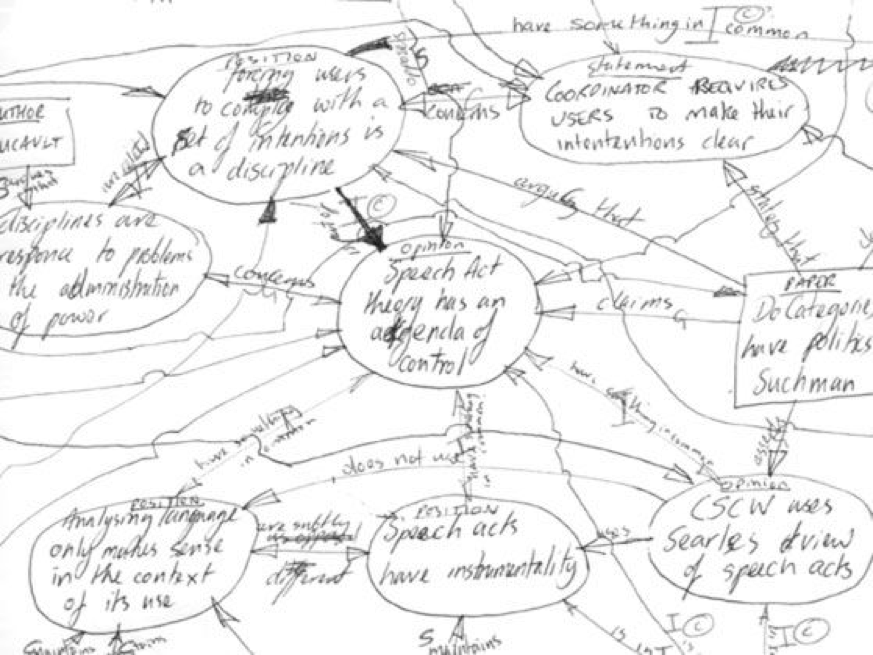
\includegraphics{img/abb2.png}
\caption{Handgezeichnete Skizze der Struktur des semantischen
Zusammenhangs des wissenschaftlichen Diskurses in der
Forschungsliteratur (aus Buckingham Shum u.a., 2007)}
\end{figure}

Dazu kann auf alte Ansätze zum Dialogue Mapping und Argument Mapping aus
der Informationswissenschaft (Conklin und Begeman, 1988, 1989; Conklin
u. a., 2001) zurückgegriffen werden (siehe Abb. 2), was die
Informationswissenschaft als genuine digitale Geisteswissenschaft
auszeichnet -- das heißt als Disziplin, die schon lange vor den Digital
Humanities auf die speziellen Bedürfnisse (nicht etwa nur auf die
(Fach-)Informationsbedürfnisse im Rahmen des Information
Retrieval-Paradigmas) von Geisteswissenschaftlern eingeht. Durch den
Ansatz zur Formalisierung bzw. Modellierung von
geisteswissenschaftlicher Forschung mit Methoden der
Wissensrepräsentation (Piotrowski, 2016) wird dabei außerdem der
Schwerpunkt auf die Unterstützung von qualitativen Methoden (Johansson,
2016) gelegt, anstatt sich -- wie in den Digital Humanities sonst üblich
-- vorwiegend auf quantitative Methoden zu konzentrieren.

Die Nützlichkeit eines solchen Formalisierungsansatzes bringen Jeff
Conklin und Michael Begeman (1988) im Kontext des Issue-Based
Information System- Ansatzes (IBIS) sehr gut auf den Punkt:

\begin{quote}
{[}T{]}he Issue-Position-Argument framework helped to focus their
thinking on the hard, critical parts of the problem, and to detect
incompleteness and inconsistency in their thinking more readliy.
{[}\ldots{}{]} They also valued the tendency for assumptions and
definitions to be made explicit.
\end{quote}

Die Notwendigkeit, beim Formalisierungsansatz explizit werden zu müssen,
führt die Geisteswissenschaftler außerdem zu formalen Modellen, die
nicht nur die Grundlage für gemeinsames Forschen mit anderen
Wissenschaftlern bildet (vgl. Piotrowski, 2016), sondern mittels eines
entsprechenden Hypertext-Werkzeugs quasi auch als Dialogpartner im
kreativen Schaffensprozess dient: „Hypertext kann eine Mittelposition
{[}zwischen lebendigem Dialog und geschriebenem Text{]}
einnehmen.``(Hammwöhner, 1997, S. 72 ff.)

Um auch auf einen alten Beitrag aus der Informatik zu verweisen, möchte
ich noch Heinz Zemanek (1992, S. 185) zitieren, der auf den besonderen
Anspruch an geisteswissenschaftliche

Wissensrepräsentation hinweist:

\begin{quote}
Diese Formalismen müssen -- das kann man nicht oft genug betonen -- den
Geisteswissenschaften äquivalent sein, und dürfen keine platten Anleihen
oder Imitationen aus den Naturwissenschaften sein; im Gegenteil: Dort,
wo solches passiert ist -- und es \emph{ist} passiert -- wird man sich
über die Rückgängigmachung den Kopf zerbrechen müssen.
\end{quote}

Die Umsetzung der Idee sollte im Bereich des Machbaren gehalten werden
können, indem auf Basis der Aufbereitung und Bereitstellung der
Forschungsliteratur anhand des Bibliothekskatalogs möglichst einfache
Werkzeuge für Annotation und Transklusion entwickelt und zur Verfügung
gestellt werden. Die Bibliothek kann so mit Denkwerkzeugen ergänzt
werden und stellt damit nicht nur Archivmaterial, Publikationen und
Forschungsinfrastruktur, sondern auch das Labor bzw. die Werkstatt für
digitale Geisteswissenschaft bereit. Die ersten Werkzeuge und
Wissensorganisationssysteme stellen beispielsweise die folgenden
grundlegenden Funktionen zur Verfügung:

\begin{itemize}
\tightlist
\item
  Transklusion von Prämissen und Konklusionen aus Publikationen für
  Argument Mapping (siehe Modellierungsansatz -- ohne Transklusion --
  von Benn und Macintosh, 2012)
\item
  Klassifikation von IBIS-Knoten mit Wissensorganisationssystemen (siehe
  beispielsweise Shum und Okada, 2008)
\item
  Verlinkung von Entitäten (Personen, Organisationen, Orte, Ereignisse)
  mit Normdaten (GND, VIAF, ORCID)
\item
  Verlinkung auf Publikationen oder auch Forschungsdaten als empirische
  Belege in Dialogue und Argument Mapping (z. B. über IBIS
  Reference-Element)
\end{itemize}

\section*{Post-Digital Humanities -- Tools, not
Toys!}\label{post-digital-humanities-tools-not-toys}

Piotrowski (2016) definiert Digital Humanities wie folgt: „The digital
humanities study the means and methods of constructing formal models in
the humanities.'' Ein Modell als Repräsentation eines
geisteswissenschaftlichen Untersuchungsgegenstands zu verstehen und
formal bedeutet soviel wie logisch kohärent, nicht mehrdeutig und
explizit. Weil Text im geisteswissenschaftlichen Bereich als Daten
behandelt werden muss (Fleer, 2016)\footnote{Text als Daten wurde unter
  anderem Anfang des Jahres beim Workshop Digitale Daten in den
  Geisteswissenschaften in der Bayerischen Akademie der Wissenschaften
  diskutiert: \url{http://dhmuc.hypotheses.org/workshop-digitale-daten}},
hat Piotrowski (2016) sicherlich recht, die wichtige Rolle von Natural
Language Processing (NLP) in den Digital Humanities und deren
Notwendigkeit als Hilfswissenschaft zu betonen. Auch ein verstärkter
Austausch mit Document Engineering bzw. Texttechnologie erscheint in
Anbetracht der immer noch zu lösenden Probleme bei der Modellierung von
Dokumenten und deren Granularität notwendig (Piotrowski, 2015).

Reiner Text kann etwa in Form eines historischen Narrativs zwar sogar
eine mechanistische Erklärung sein (vgl. Glennan, 2010, 2014), aber eben
nur als informale Beschreibung, die erstmal nicht automatisch
Computer-gestützt weiterverarbeitet werden kann und darüber hinaus
womöglich nicht logisch kohärent sondern mehrdeutig und vage ist. Das
ist dann auch nicht unbedingt redliche Geistes- bzw.
Geschichtswissenschaft, denn wie es so schön treffend im Rückentext von
Lothar Kolmer (2008) heißt: „Wer sich nicht von der Beredsamkeit der
Historiker blenden lassen will, muss das Gerüst entdecken können, das
ihre Erzählungen trägt.``

Die zuvor vorgestellten Hypertext-Werkzeuge passen sehr gut in dieses
Bild und sollen im Rahmen von Post-Digital-Humanities-Projekten die
formale Konstruktion solcher Gerüste unterstützen. Die Verwendung von
Hypertext- basierten Systemen als Denkwerkzeuge für die
Geisteswissenschaften lässt sich ab 1987 in der Geschichte der
Bibliotheks- und Informationswissenschaft beobachten, wie der Rückblick
von Erwin Welsch (1992) zeigt.

Jef Raskin (1987) kritisiert zur Blütezeit der Hypertext-Entwicklungen
-- als Hypertext-Werkzeuge auch deutlich vermehrt für
geisteswissenschaftliche Forschung entwickelt wurden (siehe Welsch,
1992) -- allerdings die vernachlässigte Benutzerfreundlichkeit der
Hypertext-Systeme. Usability Engineering wird bisher tatsächlich auch
weitgehend in den Digital Humanities vernachlässigt. Die
Informationswissenschaft könnte hier mit ihrem Bewusstsein für Aspekte
der Gebrauchstauglichkeit einen wertvollen Beitrag für die Digital
Humanities leisten (vgl. Burghardt u. a., 2015).

Um eine zielführende Werkzeugkritik durchzuführen, lohnt auch ein Blick
zurück in alte Anforderungskataloge für Hypertext-Systeme (z. B. Halasz,
1987), um nützlichere und gebrauchstauglichere Post-Digital
Humanities-Werkzeuge zu bauen. Man kann allerdings auch dafür
argumentieren, in erster Linie auf den direkten Gebrauch von
Auszeichnungs- und Modellierungssprachen zu setzen (siehe z. B. Groza u.
a., 2007) statt auf aufwändige Modellierungs- und Annotationswerkzeuge
mit grafischer Benutzeroberfläche, die sehr viel Usability Engineering
bei der Entwicklung erfordern. Hier sei passenderweise kurz auf die
Ankündigung von Ted Nelsons Vortrag Computers, Creativity, and the
Nature of the Written Word am 27. Januar 1965 im Vassar College
verwiesen (siehe Barnet, 2013, S. 73): „whole new attitudes will be
needed, and liberal- arts personages will have to learn to program,
before computers can make their real contribution to civilization.''

Mit einem programmiersprachlichen Ansatz dürfte auch der Dialog mit sich
selbst (wie

oben schon erwähnt) fließender und damit ungestörter vonstatten gehen.
Zemanek (1966, S. 141) beschreibt Programmiersprachen als Werkzeug zur
Formalisierung und Kommunikation mit sich selbst:

\begin{quote}
The language is the carrier and the implementation of ideas; since it is
very hard to handle ideas in an abstract form, the language is an
important instrument for the expression, refinement and precision of
ideas. So a programming language is also a means of communication
between a human being and himself.
\end{quote}

Wie auch immer -- vielleicht sollte man neben dem Motto von Nelson
(1996) zusätzlich auch noch die Utopie von Licklider (1960) im Auge
behalten, um nicht vom Weg zum doch recht anspruchsvollen Ziel
abzukommen:

\begin{quote}
The hope is that, in not too many years, human brains and computing
machines will be coupled together very tightly, and that the resulting
partnership will think as no human brain has ever thought and process
data in a way not approached by the information-handling machines we
know today.
\end{quote}

Die Schwierigkeit für derartige Post-Digital Humanities-Projekte besteht
nun darin, die tatsächlichen Bedürfnisse der Geisteswissenschaften zu
bedienen -- also vielmehr die Unterstützung qualitativer als
quantitativer Forschung (siehe z. B. Carvalho, 2012; Little, 2010) --
und dabei gemäß dem Motto Nelsons kurzfristige (Etappen-)Ziele
anzustreben und diese auch zu erreichen. Ob das tatsächlich möglich ist,
ohne dabei lediglich Spielzeuge anstatt richtige Werkzeuge zu bauen,
wird die zukünftige Entwicklung der Post-Digital Humanities zeigen
müssen.

\section*{Literatur}\label{literatur}

{[}Buckingham Shum u. a. 2007{]} Buckingham Shum, Simon J. ; Uren,
Victoria ; Li, Gangmin ; Sereno, Bertrand ; Mancini, Clara: Modeling
Naturalistic Argumentation in Research Literatures: Representation and
Interaction Design Issues: Research Articles. In: International Journal
of Intelligent Systems 22 (2007), Januar, Nr. 1, S. 17-47.

{[}Burghardt u. a. 2015{]} Burghardt, Manuel ; Wolff, Christian ;
Womser-Hacker, Christa: Informationsinfrastruktur und
informationswissenschaftliche Methoden in den digitalen
Geisteswissenschaften. In: Information - Wissenschaft \& Praxis 66
(2015), Januar, Nr. 5-6.

{[}Chambers 2013{]} Chambers, Sally (Hrsg.): Catalogue 2.0: the future
of the library catalogue. London : Facet Publ, 2013

{[}Conklin und Begeman 1988{]} Conklin, Jeff ; Begeman, Michael L.:
gIBIS: A Hypertext Tool for Exploratory Policy Discussion. In:
Proceedings of the 1988 ACM Conference on Computer- supported
Cooperative Work, ACM, 1988, S. 140-152.

{[}Conklin und Begeman 1989{]} Conklin, Jeff ; Begeman, Michael L.:
gIBIS: A Tool for All Reasons. In: Journal of the American Society for
Information Science 40 (1989), Mai, Nr. 3, S. 200-213.

{[}Conklin u. a. 2001{]} Conklin, Jeff ; Selvin, Albert ; Shum, Simon B.
; Sierhuis, Maarten: Facilitated Hypertext for Collective Sensemaking:
15 Years on from gIBIS. In: Proceedings of the 12th ACM Conference on
Hypertext and Hypermedia, ACM, 2001, S. 123-124.

{[}Fleer 2016{]} Fleer, Peter: Tagungsbericht: Digitale Daten in den
Geisteswissenschaften. Interdisziplinäre Perspektiven für semantische
und strukturelle Analysen, 28.01.2016 -- 29.01.2016 München. In:
H-Soz-Kult (2016).

{[}Glennan 2010{]} Glennan, Stuart: Ephemeral Mechanisms and Historical
Explanation. In: Erkenntnis 72 (2010), Nr. 2, S. 251-266.

{[}Glennan 2014{]} Glennan, Stuart: Aspects of Human Historiographic
Explanation: A View from the Philosophy of Science. S. 273-291. In:
Kaiser, Marie I. (Hrsg.) ; Scholz, Oliver R. (Hrsg.) ; Plenge, Daniel
(Hrsg.) ; Hüttemann, Andreas (Hrsg.): Explanation in the Special
Sciences: The Case of Biology and History. Dordrecht : Springer
Netherlands, 2014.

{[}Gnoli und Poli 2004{]} Gnoli, Claudio ; Poli, Roberto: Levels of
Reality and Levels of Representation. In: Knowledge Organization 31
(2004), Nr. 3, S. 151--160

{[}Halasz 1987{]} Halasz, Frank G.: Reflections on NoteCards: Seven
Issues for the Next Generation of Hypermedia Systems, ACM Press, 1987,
S. 345-365. -- ISBN 978-0-89791- 340-9.

{[}Hammwöhner 1997{]} Hammwöhner, Rainer: Offene Hypertextsysteme. Das
Konstanzer Hypertextsystem (KHS) im wissenschaftlichen und technischen
Kontext, Habilitation, 1997 6.

{[}Hennicke 2013{]} Hennicke, Steffen: Representation of Archival User
Needs using CIDOC CRM. In: Workshop Practical Experiences with CIDOC CRM
and its Extensions (CRMEX 2013), 2013

{[}Henrichs 1994{]} Henrichs, Norbert: Begriffswandel in Datenbanken:
Kontextuelle Inhaltsanalyse für Disambiguierung und ideengeschichtliche
Analyse. S. 225-239. In: Best, Heinrich (Hrsg.) ; Endres-Niggemeyer,
Brigitte (Hrsg.) ; Herfurth, Matthias (Hrsg.) ; Ohly, H. P. (Hrsg.):
Informations- und Wissensverarbeitung in den Sozialwissenschaften:
Beiträge zur Umsetzung neuer Informationstechnologien. Wiesbaden : VS
Verlag für Sozialwissenschaften, 1994.

{[}Hodel 2013{]} Hodel, Tobias: Das kleine Digitale. Ein Plädoyer für
Kleinkorpora und gegen Großprojekte wie Googles Ngram-Viewer. In:
Gugerli, David (Hrsg.) ; Hagner, Michael (Hrsg.) ; Hirschi, Caspar
(Hrsg.) ; Kilcher, Andreas B. (Hrsg.) ; Purtschert, Patricia (Hrsg.) ;
Sarasin, Philipp (Hrsg.) ; Tanner, Jakob (Hrsg.): Nach Feierabend 2013:
Digital Humanities Bd. 9. Zürich : diaphanes, 2013, S. 103--119

{[}Johansson 2016{]} Johansson, Lars-Göran: Qualitative Data and
Methods. In: Philosophy of Science for Scientists. Springer
International Publishing, 2016, S. 81-102.

{[}Kolmer 2008{]} Kolmer, Lothar: Geschichtstheorien. Paderborn : Fink,
2008 (UTB Profile 3002).

{[}Licklider 1960{]} Licklider, Joseph Carl R.: Man-Computer Symbiosis.
In: IRE Transactions on Human Factors in Electronics HFE-1 (1960), März,
S. 4-1.

{[}Licklider 1965{]} Licklider, Joseph Carl R.: Libraries of the Future.
MIT Press, 1965

{[}Mancini und Buckingham Shum 2006{]} Mancini, Clara ; Buckingham Shum,
Simon J.: Modelling Discourse in Contested Domains: A Semiotic and
Cognitive Framework. In: International Journal of Human-Computer Studies
64 (2006), November, Nr. 11, S. 1154-1171.

{[}Neil 2010{]} Neil, Benn: Using the cDnS Ontology as Upper-Level for a
Scholarly Debate Ontology. In: Frontiers in Artificial Intelligence and
Applications (2010), S. 359-372.

{[}Nelson 1965{]} Nelson, T. H.: Complex Information Processing: A File
Structure for the Complex, the Changing and the Indeterminate. In:
Proceedings of the 1965 20th National Conference, ACM, 1965, S. 84-100.

{[}Nelson 1996{]} Nelson, Ted ; Whitehead, Jim (Hrsg.): Orality and
Hypertext: An Interview with Ted Nelson. 1996. -- URL
\url{http://www.ics.uci.edu//~ejw/csr/nelson_pg.html}

{[}Nelson 2001{]} Nelson, Ted ; BBC (Hrsg.): Visionary lays into the
web. 2001. -- URL
\url{http://news.bbc.co.uk/2/hi/science/nature/1581891.stm}

{[}Nelson u. a. 2007{]} Nelson, Theodor H. ; Smith, Robert A. ;
Mallicoat, Marlene: Back to the Future: Hypertext the Way It Used to Be.
In: Proceedings of the Eighteenth Conference on Hypertext and
Hypermedia, ACM, 2007, S. 227-228.

{[}Piotrowski 2015{]} Piotrowski, Michael: Document Engineering and
Digital Humanities. In: NLP for Historical Texts: Computational
linguistics and digital humanities. URL
\url{http://nlphist.hypotheses.org/263}, Mai 2015. -- Blog

{[}Piotrowski 2016{]} Piotrowski, Michael: Digital Humanities,
Computational Linguistics, and Natural Language Processing. Lectures on
Language Technology and History. März 2016. -- URL
http://stp.lingfil.uu.se/\textasciitilde{}nivre/docs/michael\_piotrowski\_2016.pdf

{[}Pohl und Steeg 2016{]} Pohl, Adrian ; Steeg, Fabian: Zurück ins Web.
Die Entwicklung eines neuen Webauftritts für die Nordrhein-Westfälische
Bibliographie (NWBib). In: LIBREAS. Library Ideas 29 (2016). -- URL
\url{http://libreas.eu/ausgabe29/04pohl/}

{[}Raskin 1987{]} Raskin, Jef: The Hype in Hypertext: A Critique. In:
Proceedings of the ACM Conference on Hypertext, ACM, November 1987
(HYPERTEXT '87), S. 325-330 {[}Rheingold 2000{]} Rheingold, Howard:
Tools for Thought: The History and Future of Mind-Expanding Technology.
MIT Press, 2000.

{[}Stock 2016{]} Stock, Wolfgang G.: Norbert Henrichs (1935--2016):
Pionier der Informationswissenschaft in Deutschland. In: Information -
Wissenschaft \& Praxis 67 (2016), Januar, Nr. 4

{[}Sumner und Shum 1998{]} Sumner, Tamara ; Shum, Simon B.: From
Documents to Discourse: Shifting Conceptions of Scholarly Publishing.
In: Proceedings of the SIGCHI Conference on Human Factors in Computing
Systems, ACM Press /Addison-Wesley Publishing Co., 1998, S. 95-102.

{[}Treloar und Wilkinson 2008{]} Treloar, A. ; Wilkinson, R.: Rethinking
Metadata Creation and Management in a Data-Driven Research World. In:
Fourth IEEE International Conference on eScience, Dezember 2008, S.
782-789.

{[}Welsch 1992{]} Welsch, Erwin K.: Hypertext, Hypermedia, and the
Humanities. In: Library Trends 40: Electronic Information for the
Humanities (1992), Nr. 4, S. 614-646.

{[}Zemanek 1966{]} Zemanek, Heinz: Semiotics and Programming Languages.
In: Communications of the ACM 9 (1966), März, Nr. 3, S. 139143.

{[}Zemanek 1992{]} Zemanek, Heinz: Computer für die
Geisteswissenschaften, Geisteswissenschaften für den Computer. S.
166-234. In: Das geistige Umfeld der Informationstechnik, Springer,
1992.

{[}Zumstein und Stöhr 2015{]} Zumstein, Philipp ; Stöhr, Matti: Zur
Nachnutzung von bibliographischen Katalog- und Normdaten für die
persönliche Literaturverwaltung und Wissensorganisation. In: ABI Technik
35 (2015), Januar, Nr. 4 8.

%autor

\end{document}
